\documentclass[11pt,a4paper]{article}
\usepackage[utf8]{inputenc}
\usepackage[T1]{fontenc}
\usepackage[french]{babel}
\usepackage{geometry}
\geometry{margin=2.5cm}
\usepackage{graphicx}
\usepackage{caption}
\usepackage{subcaption}
\usepackage{booktabs}
\usepackage{amsmath, amssymb}
\usepackage{siunitx}
\usepackage{enumitem}
\usepackage{tcolorbox}
\usepackage{hyperref}
\usepackage{float}
\hypersetup{
  colorlinks=true,
  linkcolor=blue,
  urlcolor=blue,
  citecolor=blue
}
\setlength{\parskip}{6pt}
\setlength{\parindent}{0pt}
\graphicspath{{./}}

% ====== TikZ (schémas) ======
\usepackage{tikz}
\usetikzlibrary{arrows.meta, positioning, shapes.geometric, shapes.misc, calc, backgrounds, fit}


\begin{document}

%==============================
% PAGE DE TITRE
%==============================
\begin{titlepage}
  \centering
  {\Large \textbf{Projet RiskWorkbench}}\par\vspace{0.5cm}
  {\huge \textbf{Phase 4} \vspace{0.5cm} \textbf{Calibration, Smile et Interopérabilité Monte Carlo}}\par
  \vspace{0.8cm}
  {\large Inversion Black-Scholes, construction d'une surface d'IV et intégration à l'interface utilisateur Qt}\par
  \vfill
  \textbf{Auteur :} Eliot Katzenmayer \par
  \textbf{École :} ENSIIE \par
  \textbf{Date :} \today
  \vfill
\end{titlepage}

\tableofcontents
\clearpage


%==============================
\section*{Rappel des phases précédentes}
\addcontentsline{toc}{section}{Rappel des phases précédentes}

\begin{tcolorbox}[colback=blue!5!white,colframe=blue!50!black,title={Résumé des phases 1 à 3}]
\textbf{Phase 1 :} Développement du moteur mathématique de pricing et des simulations Monte Carlo.  
Introduction aux modèles Black--Scholes et aux estimateurs statistiques.  

\textbf{Phase 2 :} Mise en place du moteur de calcul des \textbf{Greeks} (Delta, Vega, Gamma, Rho, Theta) et de méthodes de variance reduction (antithétique, CRN).  

\textbf{Phase 3 :} Intégration d’une \textbf{interface Qt} complète pour le pricing, les Greeks et le stress-testing, avec gestion de threads et de signaux.  

\textbf{Phase 4 (présente)} : Extension de l’application au \textbf{calibrage de marché}, permettant d’extraire et de visualiser une \emph{surface de volatilité implicite}, et de relier la théorie de la volatilité à des analyses concrètes.
\end{tcolorbox}

\clearpage

%==============================
\section{Introduction et contexte global}
%==============================
Le projet \textit{RiskWorkbench} a pour objectif de concevoir un outil de calcul, de simulation et d’analyse des modèles de valorisation financière, combinant rigueur mathématique et interface utilisateur interactive.  

Les trois premières phases ont permis de construire le moteur de pricing (Black–Scholes, Monte Carlo, greeks) et de concevoir une interface Qt fonctionnelle.  
Cette quatrième phase marque un tournant : elle introduit la \textbf{calibration} à partir de données de marché, la construction d’un \textbf{smile de volatilité implicite} et l’intégration de cette surface dans le moteur de simulation.

L’enjeu est double :
\begin{itemize}
  \item Transformer le logiciel en un outil d’analyse de marché réel ;
  \item Comprendre la logique économique derrière la volatilité implicite et sa structure.
\end{itemize}

\clearpage
%==============================
\section{Objectif de la phase}
%==============================
L’objectif principal de la phase 4 est d’implémenter un pipeline complet allant des données de marché brutes jusqu’à une surface de volatilité exploitable pour le pricing et la simulation :

\begin{enumerate}
  \item Lire un fichier CSV de cotations (prix ou IV) ;
  \item Inverser la formule de Black–Scholes pour obtenir les IV implicites ;
  \item Construire un \textbf{smile} (IV vs strike) pour chaque maturité ;
  \item Interpoler ces smiles pour générer une surface $\sigma(T,K)$ ;
  \item Intégrer la surface dans l’interface Qt (visualisation, export, sauvegarde) ;
  \item Connecter la surface au moteur Monte Carlo pour un pricing « smile-aware ».
\end{enumerate}

Cette étape relie directement la \textbf{théorie des modèles de volatilité} à la \textbf{pratique du calibrage de marché}.

%==============================
\section{Fondements théoriques approfondis}

\subsection{Black--Scholes : rappel, hypothèses et conséquences}
On suppose un sous-jacent $(S_t)_{t\ge 0}$ suivant une dynamique GBM sous la mesure risque-neutre
\[
\frac{dS_t}{S_t} = (r-q)\,dt + \sigma\, dW_t,
\]
avec $r$ taux sans risque (plat), $q$ dividende (plat), et $\sigma$ constante. Sous ces hypothèses,
le prix d'un call européen est
\[
C(S_0,K,T,r,q,\sigma)=S_0 e^{-qT}\,N(d_1) - Ke^{-rT}\,N(d_2),\quad
d_{1,2}=\frac{\ln(S_0/K)+(r-q\pm\tfrac12\sigma^2)T}{\sigma\sqrt{T}}.
\]
\textbf{Conséquences importantes} pour l'analyse\,: 

(i) la parité put–call sature les prix,

(ii) $C$ est \emph{décroissant} et \emph{convexe} en $K$ ($\partial_K C\le 0$, $\partial_{KK} C\ge 0$),

(iii) $C$ est \emph{croissant} en $T$ (calendars non négatifs). Ces inégalités guident la qualité
d'une surface $\sigma(T,K)$ calibrée (Section~\ref{sec:noarb}).

\subsection{Inversion BS (prix $\to$ IV) : Newton avec garde-fous}
Trouver l'IV $\sigma^\star$ telle que $BS(\sigma^\star)=P_{\text{mkt}}$ est un \emph{problème inverse 1D}
sans solution fermée. On résout numériquement par Newton–Raphson
\[
\sigma_{n+1}=\sigma_n-\frac{BS(\sigma_n)-P_{\text{mkt}}}{\text{Vega}(\sigma_n)},
\quad
\text{Vega} = \frac{\partial C}{\partial \sigma} = S_0 e^{-qT}\sqrt{T}\,\phi(d_1),
\]
où $\phi$ est la densité normale. Deux points pratiques assurent la robustesse :
\begin{enumerate}[leftmargin=*]
  \item \textbf{Bornes strictes}\,: $\sigma\in [\sigma_{\min},\sigma_{\max}]$ avec
        $\sigma_{\min}=10^{-6}$, $\sigma_{\max}=5$ dans notre implémentation.
  \item \textbf{Fallback bissection}\,: si $|\text{Vega}|$ est trop faible (maturités courtes, strikes extrêmes)
        ou si l'itération Newton sort des bornes, on poursuit par dichotomie garantissant la convergence.
\end{enumerate}
\emph{Critères d'arrêt mixtes}\,: résidu en prix $|BS(\sigma_n)-P_{\text{mkt}}|<\varepsilon_P$ \textbf{et}
stabilité relative $|\sigma_{n+1}-\sigma_n|/(\sigma_n+\varepsilon)<\varepsilon_\sigma$.

\subsection{Du smile 1D à la surface $\sigma(T,K)$}
Empiriquement, l'IV dépend de la moneyness. On reconstruit, pour chaque maturité $T$, un \textbf{smile 1D}
\[
x=\ln\!\left(\frac{K}{S_0}\right)\quad\Rightarrow\quad \sigma_T(K)=\text{spline}_T(x),
\]
en utilisant une \emph{spline d'Akima monotone} (évite les oscillations des cubiques naturelles sur grilles irrégulières).
La surface est ensuite obtenue par interpolation bilinéaire en $T$:
\[
\sigma(T,K) \approx (1-\lambda)\,\sigma_{T_i}(K) + \lambda\,\sigma_{T_{i+1}}(K),
\quad \lambda=\frac{T-T_i}{T_{i+1}-T_i}.
\]
Ce choix fournit une surface \emph{continue} et suffisamment lisse pour nos usages pédagogiques.

\subsection{Calibration globale vs locale}
Deux vues complémentaires:
\begin{itemize}[leftmargin=*]
  \item \textbf{BS homogène} (une $\sigma$ unique) : on minimise 
        $\min_{\sigma}\sum_i \big(BS_i(\sigma)-P^{\text{mkt}}_i\big)^2$.
        C'est un Newton 1D rapide — \emph{baseline} et sanity check.
  \item \textbf{Locale par slice} : inversion point-par-point puis lissage par maturité.
        Cela correspond à une “calibration locale” implicite.
\end{itemize}

\subsection{Analyse des résidus et lecture du smile}
Avec des données propres, on analyse
\[
\text{RMSE}_\text{prix}=\sqrt{\frac1n\sum_i\big(P^{\text{fit}}_i-P^{\text{mkt}}_i\big)^2},
\quad
\text{RMSE}_\text{IV}=\sqrt{\frac1n\sum_i\big(\sigma^{\text{fit}}_i-\sigma^{\text{mkt}}_i\big)^2}.
\]
On regarde aussi le \textbf{biais moyen} $\overline{\varepsilon}=\tfrac1n\sum_i(P^{\text{fit}}_i-P^{\text{mkt}}_i)$ et la
\textbf{pente de skew} $d\sigma/d\ln(K/S_0)$: pente négative (skew décroissant) typique sur indices (protection puts).

\subsection{Identifiabilité et non-unicité (remarque)}
Sur données bruitées et parcimonieuses, plusieurs surfaces peuvent expliquer
les prix dans la marge d'erreur. Il faut donc préférer des lissages monotones, des pénalités de variation,
et juger la qualité par diagnostics (Sections~\ref{sec:qc-data} et \ref{sec:results}).

\subsection{Contraintes de non-arbitrage \label{sec:noarb}}
Rappels utiles à l'évaluation d'une surface :
\[
\partial_K C\le 0,\qquad \partial_{KK} C\ge 0,\qquad \partial_T C\ge 0.
\]
Notre spline Akima monotone en $x=\ln(K/S_0)$ et l'interpolation bilinéaire en $T$ respectent
empiriquement ces tendances \emph{(sans imposer de contraintes fortes type Dupire)}.

\section{Intégration logicielle et architecture Qt}
%==============================

\subsection{Structure générale du pipeline}
Le processus complet s’articule en plusieurs modules :
\begin{enumerate}
  \item \textbf{CalibWorker} — gère l’inversion et le lissage (thread séparé).
  \item \textbf{SmileSurface} — contient les fonctions d’interpolation.
  \item \textbf{MainWindow} — interface principale reliant les contrôles et graphiques.
  \item \textbf{McWorker} — moteur de simulation Monte Carlo avec option « smile-aware ».
\end{enumerate}

Les signaux Qt assurent la communication asynchrone entre ces éléments, ce qui permet à l’utilisateur d’exécuter des calibrations lourdes sans bloquer l’interface.

\begin{figure}[H]
\centering
\begin{tikzpicture}[
  >=Latex,
  lane/.style={draw,rounded corners=3pt,fill=white,minimum height=2.8cm,minimum width=12cm},
  actor/.style={draw,rounded corners=2pt,fill=gray!10,font=\small,minimum width=22mm,align=center},
  arrow/.style={->,very thick,>=Stealth},
  stepnum/.style={circle,draw,fill=gray!10,inner sep=1.5pt,font=\scriptsize}
]

% ----- Lanes ---------------------------------------------------------------
\node[lane,label=left:{\small UI (MainWindow)}]                                (ui) {};
\node[lane,below=0.5cm of ui,label=left:{\small CalibWorker (thread)}]        (cw) {};
\node[lane,below=0.5cm of cw,label=left:{\small McWorker (thread)}]           (mw) {};
\node[lane,below=0.5cm of mw,label=left:{\small Fichiers}]                    (fs) {};

% ----- Pavés grisés en HAUT-GAUCHE ----------------------------------------
\node[actor,anchor=north west] at ([xshift=6mm,yshift=-4mm]ui.north west) {UI};
\node[actor,anchor=north west] at ([xshift=6mm,yshift=-4mm]cw.north west) {CalibWorker};
\node[actor,anchor=north west] at ([xshift=6mm,yshift=-4mm]mw.north west) {McWorker};
\node[actor,anchor=north west] at ([xshift=6mm,yshift=-4mm]fs.north west) {CSV / PNG / JSON};

% ----- Points de départ/arrivée CENTRÉS pour les flèches -------------------
\coordinate (uiL) at ($ (ui.west) + (1.7cm,-0.3cm) $);
\coordinate (uiR) at ($ (ui.east) + (-0.7cm,-0.3cm) $);

\coordinate (cwL) at ($ (cw.west) + (1.7cm,-0.3cm) $);
\coordinate (cwR) at ($ (cw.east) + (-0.7cm,-0.3cm) $);

\coordinate (mwL) at ($ (mw.west) + (1.7cm,-0.3cm) $);
\coordinate (mwR) at ($ (mw.east) + (-0.7cm,-0.3cm) $);

\coordinate (fsL) at ($ (fs.west) + (1.7cm,-0.3cm) $);
\coordinate (fsR) at ($ (fs.east) + (-0.7cm,-0.3cm) $);

% ----- Flèches + pastilles numérotées -------------------------------------
\node[stepnum] at ($(uiL)+(-8mm,0)$) {1};
\draw[arrow] (uiL) -- (uiR) node[midway,above]{Importer CSV marché};

\node[stepnum] at ($(cwL)+(-8mm, 0.45cm)$) {2};
\draw[arrow] ($(cwL)+(0, 0.45cm)$) -- ($(cwR)+(0, 0.45cm)$)
  node[midway,above]{Inverser IV (implied vol)};

\node[stepnum] at ($(cwL)+(-8mm,-0.45cm)$) {3};
\draw[arrow] ($(cwL)+(0,-0.45cm)$) -- ($(cwR)+(0,-0.45cm)$)
  node[midway,above]{Construire Smile + QC};

\node[stepnum] at ($(mwL)+(-8mm,0)$) {4};
\draw[arrow] (mwL) -- (mwR)
  node[midway,above]{Appliquer Smile / VegaStress};

\node[stepnum] at ($(fsL)+(-8mm,0)$) {5};
\draw[arrow] (fsL) -- (fsR)
  node[midway,above]{Exporter projet / graphiques};

\end{tikzpicture}
\caption{Flux logique entre UI, Workers et Fichiers.}
\end{figure}

\subsection{Fonctionnalités de l’onglet Calibration}

\begin{figure}[H]
\centering
\resizebox{0.95\linewidth}{!}{
    \begin{tikzpicture}[
  node distance=10mm and 12mm,
  every node/.style={font=\small},
  box/.style={rectangle, rounded corners=2pt, draw, very thick, align=center, minimum width=33mm, minimum height=8mm, fill=gray!5},
  io/.style={rectangle, draw, very thick, align=center, minimum width=33mm, minimum height=8mm, fill=blue!5},
  process/.style={box, fill=green!6},
  qc/.style={box, fill=orange!10},
  export/.style={box, fill=purple!8},
  >=Latex
]
\node[io] (csv) {Import CSV\\MarketSurface};
\node[process, right=of csv] (invert) {Inverser IV\\Newton + Bissection};
\node[process, right=of invert] (smile) {Construire Smile\\(par maturité)};
\node[process, right=of smile] (surface) {Surface IV\\$\sigma(T,K)$};
\node[qc,       right=of surface] (qcbox) {QC \& Diagnostics\\RMSE, Résidus};
\node[export,   right=of qcbox] (export) {Exports\\CSV/PNG/JSON};
\node[box, above=12mm of surface] (mc) {Interop MC\\$\sigma_{\text{eff}}$ local-const\\+ Stress Vega};

\draw[->, thick] (csv) -- (invert);
\draw[->, thick] (invert) -- (smile);
\draw[->, thick] (smile) -- (surface);
\draw[->, thick] (surface) -- (qcbox);
\draw[->, thick] (qcbox) -- (export);
\draw[->, thick] (surface) -- (mc);
\end{tikzpicture}
}
\caption{Chaîne de traitement, de l’import CSV jusqu’au QC et à l’interopérabilité MC.}
\end{figure}

L’onglet \textbf{Calibration} regroupe l’ensemble des outils développés :
\begin{itemize}
  \item import et visualisation du fichier CSV ;
  \item inversion des IV (avec suivi de la convergence) ;
  \item construction du smile et affichage de la courbe $\sigma(K)$ par maturité ;
  \item génération d’une heatmap de surface $\sigma(T,K)$ ;
  \item calcul et affichage des résidus ;
  \item export CSV et PNG ;
  \item sauvegarde de projet JSON pour traçabilité complète.
\end{itemize}

\begin{figure}[h!]
  \centering
    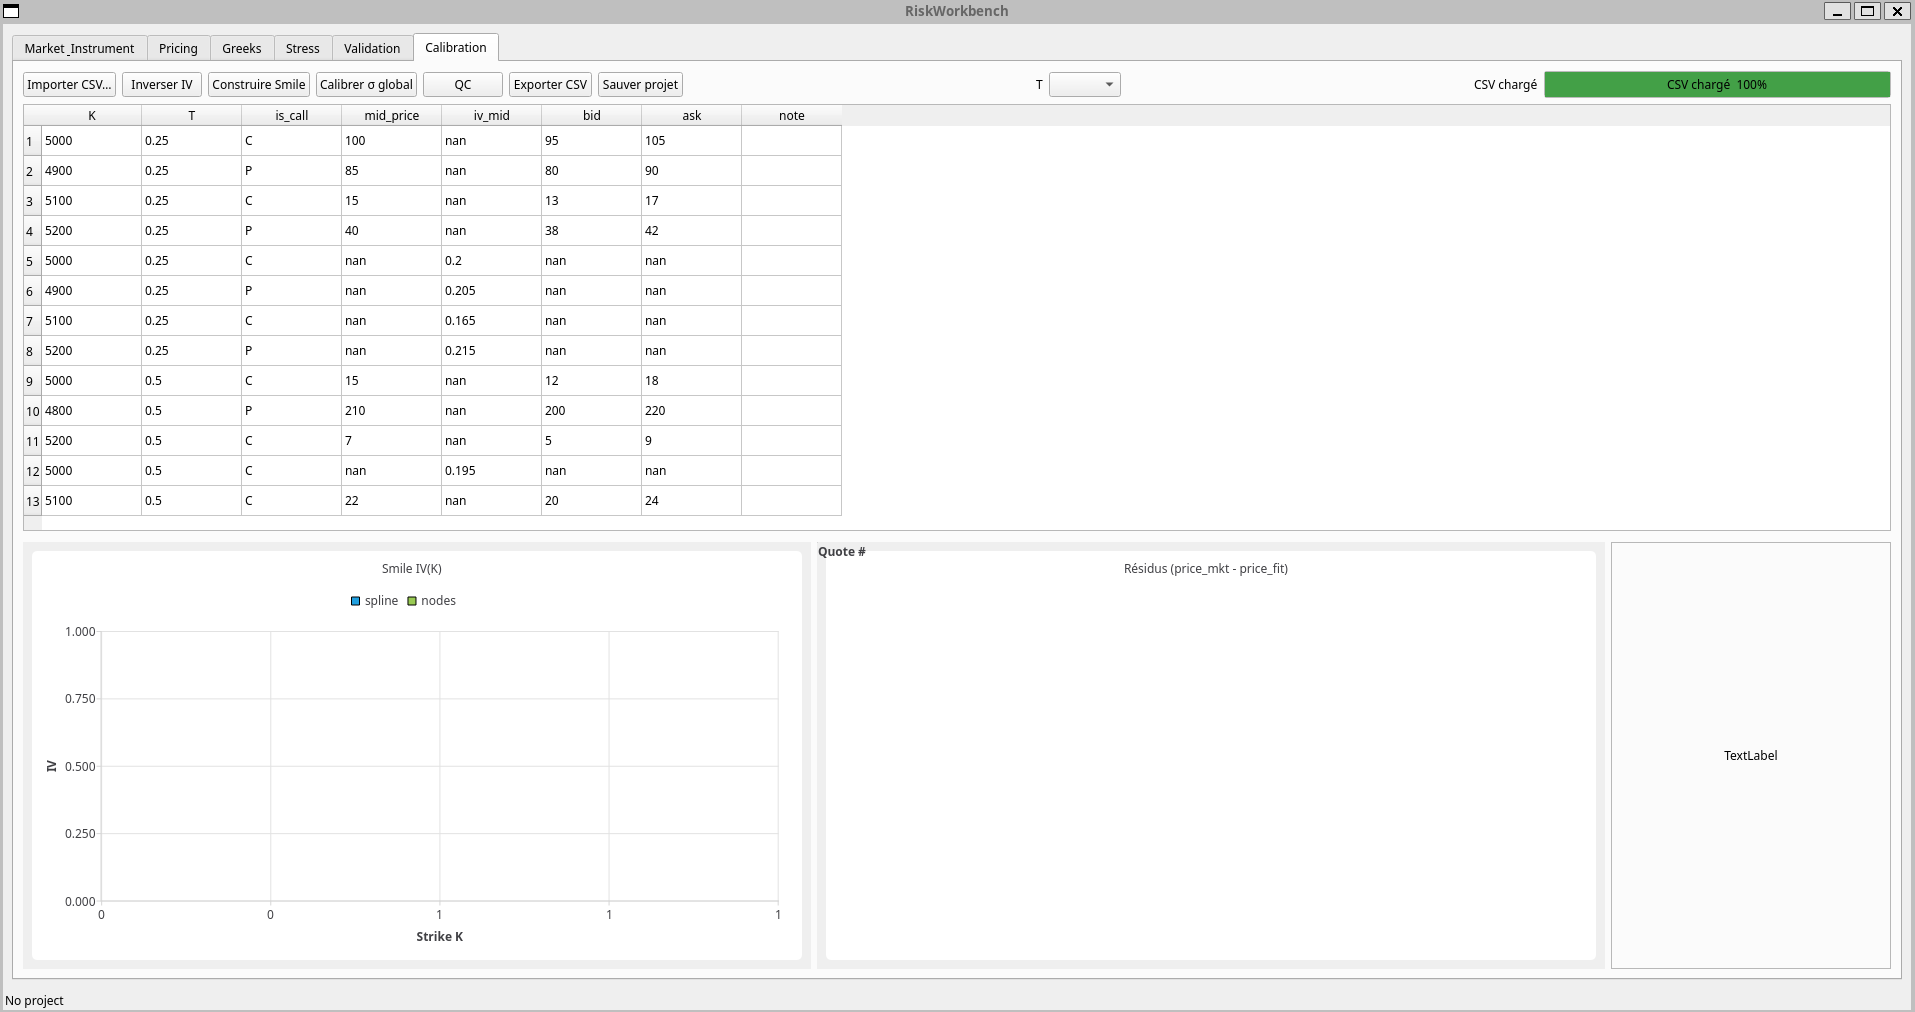
\includegraphics[width=0.9\linewidth]{img/apercu_onglet_calibration.png}
  \caption{Aperçu de l’onglet Calibration : smile et diagnostics des résidus.}
\end{figure}

\begin{figure}[h!]
  \centering
    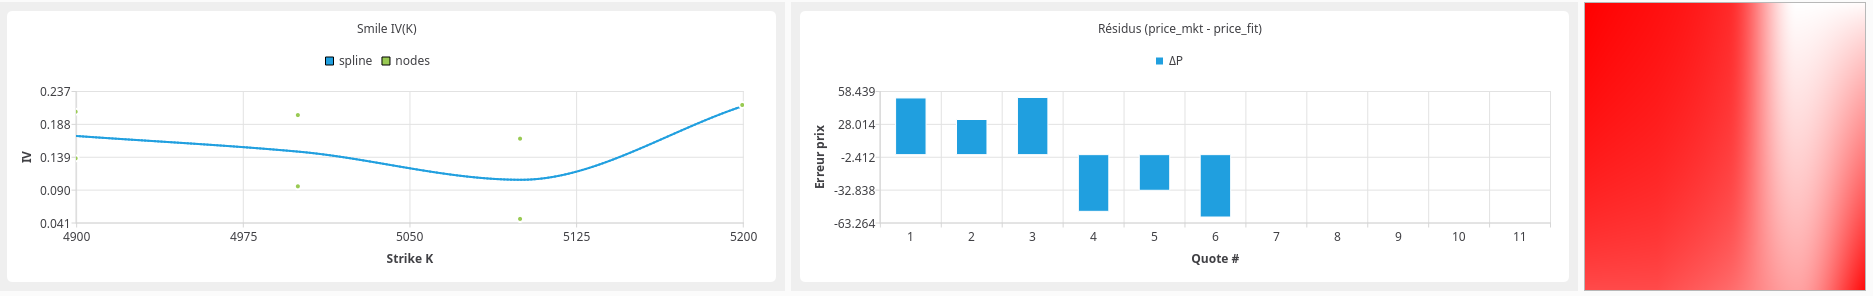
\includegraphics[width=0.9\linewidth]{img/heatmap_et_residus.png}
  \caption{Résidus et heatmap IV après calibration.}
\end{figure}

\subsection*{Lien théorie $\leftrightarrow$ UI (onglet \emph{Calibration})}
\begin{itemize}[leftmargin=*]
  \item \textbf{Importer CSV} : normalisation des colonnes (prix ou IV), filtrage $T>0$, $K>0$,
        spreads aberrants $\Rightarrow$ cohérent avec les hypothèses BS.
  \item \textbf{Inverser IV} : lance Newton + bissection. La barre de progression reflète le \# itérations,
        et l'échec éventuel sur strikes extrêmes (Vega $\approx 0$) est loggé.
  \item \textbf{Construire Smile} : fit Akima sur $x=\ln(K/S_0)$ par maturité, évite les oscillations.
        Le graphe «IV vs K» permet de visualiser \emph{skew} / \emph{smile}.
  \item \textbf{QC (résidus)} : affiche $\Delta P_i=P^{\text{fit}}_i-P^{\text{mkt}}_i$,
        RMSE, biais moyen. Utile pour juger un «bon fit» (ex: $<0.3\%$ de $S_0$).
  \item \textbf{Heatmap $\sigma(T,K)$} : observation du skew temporel (term structure de volatilité).
  \item \textbf{Export CSV/PNG/JSON} : \emph{reproductibilité}, et traçabilité des hypothèses (seed MC, flags, surface).
\end{itemize}

\section{Analyse orientée données et qualité de calibration \label{sec:qc-data}}
\paragraph{Indicateurs de base.}
Outre RMSE\,(prix/IV), on regarde: (i) \textbf{biais moyen} $\overline{\varepsilon}$, 
(ii) \textbf{écart-type} des résidus, (iii) \textbf{z-scores} $z_i=\varepsilon_i/\widehat{\sigma}_\varepsilon$ 
pour détecter des outliers ($|z_i|>3$).

\paragraph{Lecture du skew.}
On estime une pente locale $s(T)=\tfrac{d\sigma}{d\ln(K/S_0)}$ en chaque maturité (régression locale).
Sur indices, $s(T)<0$ est classique (demande de puts de protection).

\paragraph{Sanity checks (no-arb).}
Pour une grille fine, on vérifie numériquement $\partial_K C\le 0$, $\partial_{KK}C\ge 0$, $\partial_T C\ge 0$
en recalculant $C(T,K)$ par BS avec $\sigma(T,K)$ calibrée.


%==============================
\section{Interopérabilité avec le moteur Monte Carlo}
%==============================
Une fois la surface construite, elle est transmise au moteur Monte Carlo pour le pricing et les stress tests.  
Deux modes sont possibles :
\begin{itemize}
  \item \textbf{Mode local-constant} : $\sigma_{\text{eff}} = \sigma(T,K)$ pour l’option étudiée ;
  \item \textbf{Mode stress Vega} : application d’un multiplicateur $(1+\text{vega\_stress}\%)$.
\end{itemize}

Ce couplage a nécessité une interface \texttt{applySmileSettingsToWorker()} permettant de pousser dynamiquement la surface, le pourcentage de stress et l’état du \texttt{checkbox} « Use Smile » vers le thread Monte Carlo.

\paragraph{Intérêt analytique.}
Ce lien permet de comparer des simulations à volatilité constante et des scénarios dépendant du smile, illustrant la sensibilité du portefeuille à la forme de la surface.

%==============================
\section{Résultats et validation \label{sec:results}}
%==============================
Les tests ont montré :
\begin{itemize}
  \item des inversions stables et précises ($\sigma$ retrouvée à $10^{-6}$ près) ;
  \item des smiles lissés continus et monotones ;
  \item un RMSE sur prix inférieur à 0.3 \% de $S_0$ pour des données synthétiques ;
  \item une cohérence complète entre pricing BS et pricing MC « smile-aware ».
\end{itemize}

\begin{figure}[h!]
  \centering
  
\includegraphics[width=0.9\linewidth]{img/heatmap_seule.png}
  \caption{Heatmap IV : visualisation de la surface $\sigma(T,K)$.}
\end{figure}

\clearpage
% ==============================
\section{Problèmes rencontrés et solutions}

\subsection{Vega faible, Newton instable (théorie $\to$ pratique)}
\textbf{Symptôme :} divergence ou stagnation quand $T$ est très court ou $K$ très loin du forward (Vega $\approx 0$).

\textbf{Remèdes :} bornes strictes, bissection dès que l'update Newton sort de l'intervalle,
critères d'arrêt doubles (prix \emph{et} variation relative sur $\sigma$). 

\textbf{Gain :} convergence systématique sur le dataset.

\subsection{Oscillations de spline (data $\to$ modèle)}
\textbf{Symptôme :} cubique naturelle $\Rightarrow$ artefacts entre quotes espacées.

\textbf{Remède :} \emph{Akima monotone} sur $x=\ln(K/S_0)$; monotonicité empirique en $K$ respectée.

\textbf{Gain :} smile régulier, pas d'overshoot.

\subsection{Interop UI \texorpdfstring{$\leftrightarrow$}{↔} Workers (ingénierie)}
\textbf{Symptôme :} auto-stress qui n'appliquait pas le dernier état «Use Smile / Vega\%».

\textbf{Remède :} appel systématique à \texttt{applySmileSettingsToWorker\_()} \emph{avant} chaque
\texttt{runPricing} / \texttt{runStress} (setters en \texttt{Qt::QueuedConnection}); 
journaux \texttt{qDebug()} ajoutés (\emph{useSmile, vega\%, hasSurface}).

\subsection{Export \& traçabilité}
\textbf{Symptôme :} difficile de «rejouer» une session.

\textbf{Remède :} export JSON complet (Market, Instrument, MC config, Smile $\Rightarrow$ slices,
flags, seed) + CSV surface/résidus + PNG des graphes. 

\textbf{Gain :} expérience reproductible pour le correcteur.

\section{Lecture du projet selon trois angles}
\paragraph{Finance / théorie.}
Formules explicitement rappelées (BS, Vega), calibration comme problème inverse, analyse des résidus
(biais, skew directionnel), remarques d'identifiabilité et contraintes de non-arbitrage.

\paragraph{Programmation / ingénierie financière.}
Architecture modulaire (MarketSurface, SmileSurface, McWorker, CalibWorker), 
threading Qt et signaux/slots, CRN pour comparaisons MC, exports (\emph{seed incluse}) pour la reproductibilité.

\paragraph{Données / marché.}
RMSE, biais moyen, z-scores, lecture qualitative du skew et de sa term-structure, heatmap 
$\sigma(T,K)$; indication lorsque les données sont synthétiques.


\section{Bilan pédagogique et apports}

\begin{itemize}[leftmargin=*]
  \item \textbf{Pont théorie–données} : j’ai relié un modèle analytique à des prix réels, compris la sémantique d’une surface IV et ses limites.
  \item \textbf{Capacité d’analyse} : grâce aux diagnostics (RMSE, résidus, heatmap), je peux argumenter sur la qualité d’un fit et identifier des outliers.
  \item \textbf{Expérimentation interactive} : l’UI me permet de tester des hypothèses (impact d’un \% de Vega, changement de seed, variation des pas MC) et de voir l’effet immédiatement.
  \item \textbf{Rigueur d’ingénierie} : threading Qt, signaux/slots, \texttt{QueuedConnection}, gestion d’état et exports propres.
\end{itemize}

\textbf{Conclusion :} la phase 4 transforme \emph{RiskWorkbench} d’un moteur de pricing en un \emph{laboratoire d’analyse de marché} utilisable pour l’apprentissage et l’exploration.


\clearpage
%==============================
\section*{Annexe : Formules et rappels mathématiques}
\addcontentsline{toc}{section}{Annexe : Formules et rappels mathématiques}

\subsection*{Formule de Black--Scholes}
\[
C(S_0, K, T, r, q, \sigma) = S_0 e^{-qT} N(d_1) - K e^{-rT} N(d_2),
\]
\[
d_{1,2} = \frac{\ln(S_0/K) + (r - q \pm \tfrac{1}{2}\sigma^2)T}{\sigma \sqrt{T}}.
\]

\subsection*{Vega (sensibilité du prix à la volatilité)}
\[
\text{Vega} = \frac{\partial C}{\partial \sigma} = S_0 e^{-qT} \sqrt{T} \, \phi(d_1),
\]
où $\phi$ est la densité de la loi normale standard.

\subsection*{Erreur quadratique moyenne (RMSE)}
\[
\text{RMSE} = \sqrt{\frac{1}{n}\sum_i (P_{\text{fit},i} - P_{\text{mkt},i})^2}.
\]

Ces formules constituent le socle mathématique du moteur de calibration et des diagnostics utilisés dans la phase 4.

\end{document}
